%%%%%%%%%%%%%%%%%%%%%%%%%%%%%%%%%%%%%%%%%%%%%%%%%%%%%%%%%%%%%%%%%%%%%%%%%%%%
%DIF LATEXDIFF DIFFERENCE FILE
%DIF DEL GulfStreamAguR1.tex   Mon Nov 23 10:33:58 2015
%DIF ADD GulfStreamAgu.tex     Tue Jan  5 14:37:44 2016
% AGUtmpl.tex: this template file is for articles formatted with LaTeX2e,
% Modified July 2014
%
% This template includes commands and instructions
% given in the order necessary to produce a final output that will
% satisfy AGU requirements.
%
% PLEASE DO NOT USE YOUR OWN MACROS
% DO NOT USE \newcommand, \renewcommand, or \def.
%
% FOR FIGURES, DO NOT USE \psfrag or \subfigure.
%
%%%%%%%%%%%%%%%%%%%%%%%%%%%%%%%%%%%%%%%%%%%%%%%%%%%%%%%%%%%%%%%%%%%%%%%%%%%%
%
% All questions should be e-mailed to latex@agu.org.
%
%%%%%%%%%%%%%%%%%%%%%%%%%%%%%%%%%%%%%%%%%%%%%%%%%%%%%%%%%%%%%%%%%%%%%%%%%%%%
%
% Step 1: Set the \documentclass
%
% There are two options for article format: two column (default)
% and draft.
%
% PLEASE USE THE DRAFT OPTION TO SUBMIT YOUR PAPERS.
% The draft option produces double spaced output.
%
% Choose the journal abbreviation for the journal you are
% submitting to:

% jgrga JOURNAL OF GEOPHYSICAL RESEARCH
% gbc   GLOBAL BIOCHEMICAL CYCLES
% grl   GEOPHYSICAL RESEARCH LETTERS
% pal   PALEOCEANOGRAPHY
% ras   RADIO SCIENCE
% rog   REVIEWS OF GEOPHYSICS
% tec   TECTONICS
% wrr   WATER RESOURCES RESEARCH
% gc    GEOCHEMISTRY, GEOPHYSICS, GEOSYSTEMS
% sw    SPACE WEATHER
% ms    JAMES
% ef    EARTH'S FUTURE
% ea    EARTH AND SPACE SCIENCE
%
%
%
% (If you are submitting to a journal other than jgrga,
% substitute the initials of the journal for "jgrga" below.)
%\documentclass[draft,jgrga]{agutex2015}

\documentclass[draft,grl]{agutex2015}
% To create numbered lines:

% If you don't already have lineno.sty, you can download it from
% http://www.ctan.org/tex-archive/macros/latex/contrib/ednotes/
% (or search the internet for lineno.sty ctan), available at TeX Archive Network (CTAN).
% Take care that you always use the latest version.

% To activate the commands, uncomment \usepackage{lineno}
% and \linenumbers*[1]command, below:


\usepackage[plain]{fancyref}
\usepackage{lineno}
\usepackage{url}
\linenumbers*[1]
%  To add line numbers to lines with equations:
%  \begin{linenomath*}
%  \begin{equation}
%  \end{equation}
%  \end{linenomath*}
%%%%%%%%%%%%%%%%%%%%%%%%%%%%%%%%%%%%%%%%%%%%%%%%%%%%%%%%%%%%%%%%%%%%%%%%%
% Figures and Tables
%
%
% DO NOT USE \psfrag or \subfigure commands.
%
%
%  Uncomment the following command to include .eps files
%  (comment out this line for draft format):
\usepackage[]{graphicx}

\usepackage{setspace,caption}
\captionsetup[table]{font={stretch=1.2}}     %% change 1.2 as you like
\captionsetup[figure]{font={stretch=1.2}}

%
%  Uncomment the following command to allow illustrations to print
%   when using Draft:
\setkeys{Gin}{draft=false}
%
% Substitute one of the following for [dvips] above
% if you are using a different driver program and want to
% proof your illustrations on your machine:
%
% [xdvi], [dvipdf], [dvipsone], [dviwindo], [emtex], [dviwin],
% [pctexps],  [pctexwin],  [pctexhp],  [pctex32], [truetex], [tcidvi],
% [oztex], [textures]
%
% See how to enter figures and tables at the end of the article, after
% references.
%
%% ------------------------------------------------------------------------ %%
%
%  ENTER PREAMBLE
%
%% ------------------------------------------------------------------------ %%

% Author names in capital letters:
\authorrunninghead{KLYMAK ET AL.}

% Shorter version of title entered in capital letters:
\titlerunninghead{GULF STREAM SUBMESOSCALE STREAMERS}

%Corresponding author mailing address and e-mail address:
%\authoraddr{Corresponding author: A. B. Smith,
%Department of Hydrology and Water Resources, University of
%Arizona, Harshbarger Building 11, Tucson, AZ 85721, USA.
%(a.b.smith@hwr.arizona.edu)}

%DIF PREAMBLE EXTENSION ADDED BY LATEXDIFF
%DIF UNDERLINE PREAMBLE %DIF PREAMBLE
\RequirePackage[normalem]{ulem} %DIF PREAMBLE
\RequirePackage{color}\definecolor{RED}{rgb}{1,0,0}\definecolor{BLUE}{rgb}{0,0,1} %DIF PREAMBLE
\providecommand{\DIFadd}[1]{{\protect\color{blue}\uwave{#1}}} %DIF PREAMBLE
\providecommand{\DIFdel}[1]{{\protect\color{red}\sout{#1}}}                      %DIF PREAMBLE
%DIF SAFE PREAMBLE %DIF PREAMBLE
\providecommand{\DIFaddbegin}{} %DIF PREAMBLE
\providecommand{\DIFaddend}{} %DIF PREAMBLE
\providecommand{\DIFdelbegin}{} %DIF PREAMBLE
\providecommand{\DIFdelend}{} %DIF PREAMBLE
%DIF FLOATSAFE PREAMBLE %DIF PREAMBLE
\providecommand{\DIFaddFL}[1]{\DIFadd{#1}} %DIF PREAMBLE
\providecommand{\DIFdelFL}[1]{\DIFdel{#1}} %DIF PREAMBLE
\providecommand{\DIFaddbeginFL}{} %DIF PREAMBLE
\providecommand{\DIFaddendFL}{} %DIF PREAMBLE
\providecommand{\DIFdelbeginFL}{} %DIF PREAMBLE
\providecommand{\DIFdelendFL}{} %DIF PREAMBLE
%DIF END PREAMBLE EXTENSION ADDED BY LATEXDIFF

\begin{document}

%% ------------------------------------------------------------------------ %%
%
%  TITLE
%
%% ------------------------------------------------------------------------ %%


\title{Submesoscale streamers exchange water on the north wall of the Gulf Stream}
%
% e.g., \title{Terrestrial ring current:
% Origin, formation, and decay $\alpha\beta\Gamma\Delta$}
%

%% ------------------------------------------------------------------------ %%
%
%  AUTHORS AND AFFILIATIONS
%
%% ------------------------------------------------------------------------ %%


%Use \author{\altaffilmark{}} and \altaffiltext{}

% \altaffilmark will produce footnote;
% matching \altaffiltext will appear at bottom of page.

% \authors{A. B. Smith,\altaffilmark{1}
% Eric Brown,\altaffilmark{1,2} Rick Williams,\altaffilmark{3}
% John B. McDougall\altaffilmark{4}, and S. Visconti\altaffilmark{5}}

%\altaffiltext{1}{Department of Hydrology and Water Resources,
%University of Arizona, Tucson, Arizona, USA.}

%\altaffiltext{2}{Department of Geography, Ohio State University,
%Columbus, Ohio, USA.}

%\altaffiltext{3}{Department of Space Sciences, University of
%Michigan, Ann Arbor, Michigan, USA.}

%\altaffiltext{4}{Division of Hydrologic Sciences, Desert Research
%Institute, Reno, Nevada, USA.}

%\altaffiltext{5}{Dipartimento di Idraulica, Trasporti ed
%Infrastrutture Civili, Politecnico di Torino, Turin, Italy.}

\author{Jody M. Klymak\altaffilmark{1}}
\author{R. Kipp Shearman\altaffilmark{2}}
\author{Jonathan Gula\altaffilmark{3}}
\author{Craig M. Lee\altaffilmark{4}}
\author{Eric A. D'Asaro\altaffilmark{4}}
\author{Leif N. Thomas\altaffilmark{5}}
\author{Ramsey R. Harcourt\altaffilmark{4}}
\author{Andrey Y. Shcherbina\altaffilmark{4}} 
\author{Miles A. Sundermeyer\altaffilmark{6}}
\author{Jeroen Molemaker\altaffilmark{7}} 
\author{James C. McWilliams\altaffilmark{7}}

\altaffiltext{1}{University of Victoria, Victoria, British Columbia, Canada}
\altaffiltext{2}{Oregon State University, Corvallis, Oregon, USA}
\altaffiltext{3}{Laboratoire d'Oc\'eanographie Physique et Spatiale, Universit\'e de Brest, Brest, France}
\altaffiltext{4}{Applied Physics Laboratory, University of Washington, Seattle, Washington USA}
\altaffiltext{5}{Stanford University, Stanford, California, USA}
\altaffiltext{6}{University of Massachusetts Dartmouth, Dartmouth, Massachusetts, USA}
\altaffiltext{7}{University of California, Los Angeles, California, USA }
\clearpage 



%% ------------------------------------------------------------------------ %%
%
%  ABSTRACT
%
%% -------------------------------------------s---------------------------- %%

% >> Do NOT include any \begin...\end commands within
% >> the body of the abstract.

\begin{abstract}
The Gulf Stream is a major conduit of warm surface water from the tropics to the subpolar North Atlantic.  Here we observe and simulate a sub-mesoscale ($<20$ km) mechanism by which the Gulf Stream exchanges water with subpolar water to the north. The front exhibits a sharp temperature-salinity contrast, with distinct ``mixed'' water between the two water masses  2 and 4 km wide.  This mixed water does not increase downstream despite substantial energy available for mixing.  A series of ``streamers'' detrain this water at the crest of meanders. Subpolar water replaces the mixed water and resharpens the front. The water mass exchange  accounts for a northwards flux of salt of $0.8-5\ \mathrm{psu\ m^2s^{-1}}$, (large-scale diffusivity $O(100\ \mathrm{m^2s^{-1}})$). This is similar to bulk-scale flux estimates of $1.2\ \mathrm{psu\ m^2s^{-1}}$, and supplies fresh water to the Gulf Stream required for the production of 18-degree subtropical mode water.
\end{abstract}

\keypoints{
%\begin{list}
  \item Lateral detrainment clearly observed from North Wall at depth.  
  \item Salt flux similar to bulk estimates. 
  \item  Detrained water is from a distinct partially mixed water class. 
%\end{list} 
}
%% ------------------------------------------------------------------------ %%
%
%  BEGIN ARTICLE
%
%% ------------------------------------------------------------------------ %%

% The body of the article must start with a \begin{article} command
%
% \end{article} must follow the references section, before the figures
%  and tables.

\begin{article}

%% ------------------------------------------------------------------------ %%
%
%  TEXT
%
%% ------------------------------------------------------------------------ %%

\section{Introduction}

The Gulf Stream (GS) is the western boundary current of the North Atlantic subtropical wind-driven circulation.  It separates from Cape Hatteras where it flows eastward into the North Atlantic.  As it flows, it loses heat to  the atmosphere and by mixing with the cold water in the subpolar gyre to the north.  It also becomes fresher, an observation that can only be explained by entrainment of fresh water from the north \citep{joyceetal13}.  As it entrains water, the GS  increases its eastward transport by approximately $40-80\ \mathrm{m^2s^{-1}}$ \citep{johnsetal95}.   

The GS has a sharp density front that outcrops at the surface. It also has a sharp temperature and salinity front, as has been demonstrated at the surface from shipboard surveys \citep{fordetal52} and satellite images \citep{churchilletal89}. The sharpness of the front beneath the surface has been less-clear, and requires high-resolution lateral sampling to resolve. The front has a sharp potential vorticity gradient \citep{rajamonyetal01}, and such gradients act as a barrier to lateral mixing \citep{marshalletal06,naveiraetal11}.  Despite this  barrier, property budgets indicate that there is significant exchange across the north wall \citep{joyceetal13}, and that entrainment of fresh water is necessary to create the dynamically important ``18-degree water'' that fills much of the upper Sargasso Sea. 

The mechanisms controlling this lateral mixing have not been identified. There are large eddies that periodically pinch off the GS and carry warm water to the north. However, some of these are re-entrained into the GS and do not result in a net exchange. Instead, tracer budgets across the front appear to be dominated by small, submesoscale processes \citep{boweretal85}. To date some of the best direct evidence for cross-front exchange consists of the trajectories of density-following floats placed at the north wall \citep{bowerrossby89,bowerlozier94}.  These floats were observed to regularly detrain from the GS, such that of 95 floats, 26 stayed in the GS, 7 were detrained in rings, and 62 were detrained by mechanisms other than rings \citep{bowerlozier94}.  Kinematic theories have been examined to explain the detrainment of the floats \citep{flierletal87,stern85,prattetal95}, and the similarity to satellite images of ``streamers'' of warm water detraining from the Gulf Stream has been noted.  However, direct observations of the  processes as it occurs at depth have been lacking.  

Here we point out that the density front is accompanied by a sharp (<5 km wide) and persistent temperature-salinty front along isopycnals.  We also present indirect evidence that there is small-scale mixing ($<$0.5 km) on the northern cyclonic side of the GS, and that the mixed water periodically peels off the GS in thin (5-10 km wide) ``streamers''. We describe our experiment, and the observations that it yielded before briefly discussing the implications.

\section{Methods}

 In March 2012 we made high-resolution measurements of the north wall of the GS from 66 W to 60 W (\fref{fig:SatOverviewSectD}), about 850 km east of where the GS separates from the North American continental slope.   A Lagrangian float \citep{dasaro03} was placed in the Gulf Stream front based on a brief cross-stream survey, and programmed to match the density of the surface mixed layer (upper 30 m).  The float moved downstream at a mean speed of 1.4 $\mathrm{m\,s^{-1}}$.  The \emph{R/V Knorr} tracked the float and deployed a Chelsea Instruments TriAxus that  collected temperature, salinity, and pressure (CTD) on a 200-m deep sawtooth with approximately 1-km lateral spacing in a 10-km box-shaped pattern relative to the float (\fref{fig:SatOverviewSectD}, magenta).  \emph{R/V Atlantis} performed larger cross sections approximately 30 km across the front, trying to intercept the float on each front crossing.  \emph{R/V Atlantis} was deploying a Rolls Royce Marine Moving Vessel Profiler equipped with a CTD that profiled to 200 m approximately every 1 km.  Both ships had a 300 kHz RDI Acoustic Doppler Current Profiler (ADCP) collecting currents on 2-m vertical scale averaged every 5 minutes (approximately 1 km lateral scale), collected and processed using UHDAS and CODAS (http://currents.soest.hawaii.edu \cite{firingetal12}).  Velocities are put into a float-following frame as a proxy for along- and across-front, with $u$ being defined as along the floats path, and $v$ as perpendicular to the path and to the north.  Velocity data at 2-m vertical resolution reached about 130 m, and were supplemented at deeper depths with data from 75 kHz RDI ADCPs, with 8-m vertical resolution.  

\begin{figure*}[htbp]
  \centering
    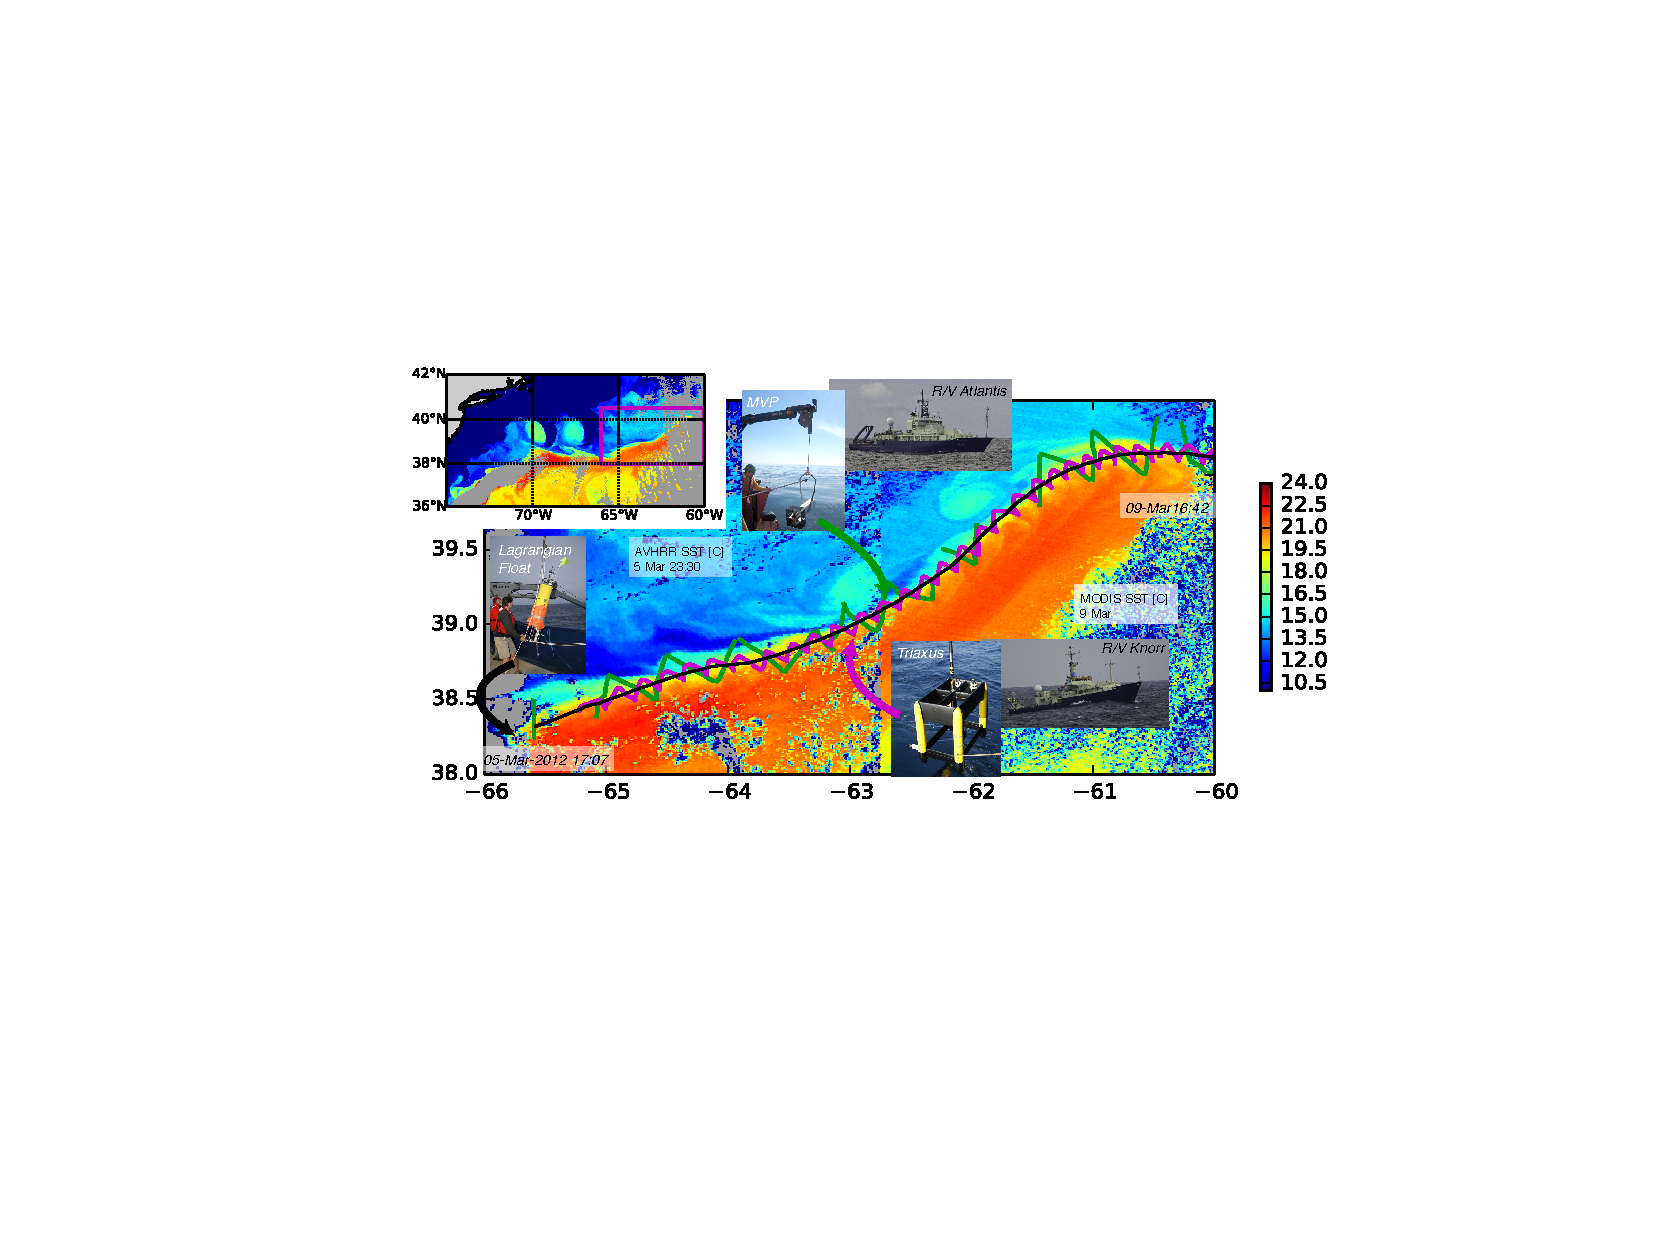
\includegraphics[width=\textwidth]{./SatOverviewSecDTry2.pdf}
   \caption{ The experimental design  Inset: The experiment site on the north wall of the Gulf Stream, between 66 and 60 W, as shown in an AVHRR satellite image of sea surface temperature (SST).  Main:  Detailed SST image composed from two satellite images.    The GS is warm and delineated by a sharp front.  The small sub-mesoscale structures north of the front are the focus of this paper.  The satellite images are a composite from early in the observation period (AVHRR 6 Mar), and late (MODIS, 9 Mar).  A Lagrangian float was deployed in the front (black curve), and the ship tracks bracketed the float's position (green: \emph{R/V Atlantis}, magenta: \emph{R/V Knorr}). \emph{R/V Atlantis} cross-sections labeled a-d are shown in \fref{fig:SalDFirstStreamer}a-d.  }\label{fig:SatOverviewSectD}
\end{figure*}

Data were interpolated onto a cube delineated by depth surfaces by creating a two-dimensional interpolation onto a grid via Delauney triangulation at each depth; no extrapolation was performed.  Data on the $26.25\ \mathrm{kg\,m^{-3}}$ isopycnal were assembled at each grid point by finding the first occurrence of that isopycnal in depth.  
Potential vorticity is calculated from the three-dimensional grid as
\begin{equation}
  q = -\frac{g}{\rho_0}\left(\nabla \times\mathbf{u}+\mathbf{f}\right) \cdot \nabla\rho,
\end{equation}
where $f$ is the Coriolis frequency, $g$ the gravitational acceleration. The bracketed term is twice the angular velocity, including the planet's rotation, and the gradient of density represents the stretching or compression of the water column.  In the GS, the potential vorticity is dominated by contributions from the vertical density gradient and the cross-stream gradient of the along-stream velocity, which was used to calculate potential vorticity from two-dimensional sections:
\begin{equation}
  q \approx N^2\left(-\frac{\partial u}{\partial y}+f\right).
\end{equation}

At select times during the float evolutions, fluorescein dye releases (100 kg per release) were conducted at depth as close as possible to the float.  Dye was pumped down a hose to a tow package deployed off the side of the ship, consisting of a CTD and a dye diffuser.  Prior to injection, the dye was mixed with alcohol and ambient sea water to bring it to within \DIFdelbegin \DIFdel{$0.001\ \mathrm{kg m^-3}$ }\DIFdelend \DIFaddbegin \DIFadd{$0.001\ \mathrm{kg m^{-3}}$ }\DIFaddend of the float's target density. Initial dimensions of the dye streak were $\approx$1 km along-stream, $\approx$100 m cross-stream (after wake adjustment), and ranging from 1 - 5 m in the vertical. The TriAxus system on the \emph{R/V Knorr} tracked the fluorescein from its CTD package.  

Numerical simulations of the GS were performed with the Regional Oceanic Modeling System \citep[ROMS][]{shchepetkinmcwilliams05}. The simulation has a horizontal resolution of 500m and 50 vertical levels. The model domain spans 1,000 km by 800 km and covers a region of the GS downstream from its separation from the U.S. continental slope. Boundary conditions are supplied by a sequence of two lower-resolution simulations that span the entire GS region and the Atlantic basin, respectively. The simulation is forced by daily winds and diurnally modulated surface fluxes. The modelling approach is described in detail in \citet{gulaetal15}.

Neutrally buoyant Lagrangian (flow-following) particles were seeded into the model at a time $t0$ and advected both backwards and forwards in time by the model velocity fields without additional dispersion from the model's mixing processes \citep{gulaetal14}. A 4th-order Runge-Kutta method with a time step  $dt = 1\ \mathrm{s}$ is used to compute particle advection. Velocity and tracer fields are interpolated at the positions of the particles using cubic spline interpolation in both the horizontal and vertical directions.  We linearly interpolate hourly outputs in time from the simulation to get sufficiently frequent and temporally-smooth velocity sampling for accurate parcel advection.

\section{Observations}

During these observations, the GS had a shallow meander crest at 65 W (\fref{fig:SatOverviewSectD}b)  followed by a long concave region (63 W) and then another large  crest (61 W).  Satellite measurements show the sharp temperature changes across the front, superimposed with thin intermediate-temperature (15-18$^o$C) streamers detraining to the north at approximately 65 W, 64 W, and at the crest of the large meander at 61 W.  An older streamer that has rolled up can also be seen at 62 W.  The ships passed through the three newer streamers providing a detailed observation of their underwater structure.  

The front consists of density surfaces that slope up towards the north (\fref{fig:SalDFirstStreamer}a-d).  The water along density surfaces is saltier (and warmer) in the GS, and fresher (and colder) to the north. The transition between the two water masses is remarkably abrupt, occurring over less than 5-km.  This sharpness persisted from the western-most section during the cruise (71.5 W) to the eastern-most (60.5 W). Some cross sections show lateral interleaving of salinity north of the front \DIFaddbegin \DIFadd{deeper than 70 m }\DIFaddend (\fref{fig:SalDFirstStreamer}a) with approximately 5-km wide salinity anomalies ($S \approx 36.15\ \mathrm{psu}$).  These anomalies move slower than the front (\fref{fig:SalDFirstStreamer}e), and have high potential vorticity that is normally associated with the front (\fref{fig:SalDFirstStreamer}i).  \DIFaddbegin \DIFadd{The surface signature of the streamers (as seen in }\fref{fig:SatOverviewSectD}\DIFadd{b) can be also seen in these cross-sections as saltier ``surface'' water (}\fref{fig:SalDFirstStreamer}\DIFadd{a-d)), but the T/S characteristics are not as distinct because of cooling by the atmosphere.  
}\DIFaddend 

The temperature-salinity (T/S) relationship of this data shows the contrast between the GS and the subpolar water as two distinct modes (\DIFdelbegin %DIFDELCMD < \fref{fig:ComposeTSfigNew}%%%
\DIFdel{a}\DIFdelend \DIFaddbegin \fref{fig:TSDensityPlot}\DIFaddend , labeled ``North'' and ``Gulf Stream''), except near the surface where the water masses are strongly affected by the atmosphere.  For the deeper water, there is a third distinct population between the two larger modes in T/S space that represents the water in the salinity anomalies, \DIFdelbegin \DIFdel{and }\DIFdelend \DIFaddbegin \DIFadd{that }\DIFaddend we have labelled as ``streamers''.  The distinctness in T/S space of the streamers indicates that after the GS and subpolar waters mixed, the partially mixed water continued to mix, condensing it in T/S space so that it forms an almost-separate water mass. \DIFaddbegin \DIFadd{Below, we further differentiate water in this T/S class as either ``attached'' to the GS or ``detached''.   
}\DIFaddend 

Looking at the GS in plan view along the $\sigma_{\theta} = 26.25\ \mathrm{kg\,m^{-3}}$ isopycnal (\DIFdelbegin %DIFDELCMD < \fref{fig:ComposeTSfigNew}%%%
\DIFdel{b}\DIFdelend \DIFaddbegin \fref{fig:IsoSurface}\DIFadd{a}\DIFaddend ) we see the mixed water that that makes up the streamers is connected along the length of our observations, with a width that averages just less than 4km wide (\DIFdelbegin %DIFDELCMD < \fref{fig:ComposeTSfigNew}%%%
\DIFdel{c}\DIFdelend \DIFaddbegin \fref{fig:IsoSurface}\DIFadd{b}\DIFaddend ). The first streamer (64.5 W) is horizontally connected over 100 km, and is about 5 km wide, and at least 150 m deep.  Where the streamer is the most detached (\fref{fig:SalDFirstStreamer}a) the main front is the sharpest of the \DIFdelbegin \DIFdel{4 }\DIFdelend \DIFaddbegin \DIFadd{four }\DIFaddend cross sections.    Downstream of this streamer, the mixed water thins before the eastern meander (60.5 W) where there is a second streamer.  Further downstream, the mixed water almost disappears by the last cross-section (59 W), and there is evidence of a streamer to the north of the sampling pattern.  

We can estimate the rate of detrainment from the first streamer (64.5 W). It starts on the fast side of the front with water flowing approximately \DIFdelbegin \DIFdel{$0.25\ \mathrm{m\,s^{-1}}$ }\DIFdelend \DIFaddbegin \DIFadd{$0.1-0.25\ \mathrm{m\,s^{-1}}$ }\DIFaddend faster than the float (\fref{fig:SalDFirstStreamer}h). Upstream, where it is detached (\fref{fig:SalDFirstStreamer}e), it is flowing almost \DIFdelbegin \DIFdel{$0.5\ \mathrm{m\,s^{-1}}$ }\DIFdelend \DIFaddbegin \DIFadd{$0.2-0.5\ \mathrm{m\,s^{-1}}$ }\DIFaddend slower than the float.  \DIFdelbegin \DIFdel{A 5-km wide and 150-m deep streamer ,  with a relative velocity of $0.75\ \mathrm{m\,s^{-1}}$ represents a rate of detrainment of over $0.5\times10^{6}\, \mathrm{m^{3}\,s^{-1}}$}\DIFdelend \DIFaddbegin \DIFadd{Integrating the transport relative to the attached water just downstream, we see that the streamer detrains $0.2-0.25 \times 10^6\ \mathrm{m^3\,s^{-1}}$ of water (}\fref{fig:IsoSurface}\DIFadd{c).  This estimate is quite rough, given that the fully detached streamer was only sampled three times, the arbitrary division between ``attached'' and ``detached'' water, and the overall inhomogeneity of the water mass, but it serves as a rough estimate until better measurements can be made}\DIFaddend .  

The streamers move up through the water column along isopycnals and the water parcels are stretched vertically. The streamer in \fref{fig:SalDFirstStreamer}a has risen along isopycnals from 140 m deep (\fref{fig:SalDFirstStreamer}d)  to less than 40 m deep \DIFaddbegin \DIFadd{(}\fref{fig:SalDFirstStreamer}\DIFadd{a)}\DIFaddend , and titled somewhat as it has done so.   The velocity anomaly is about $0.75\ \mathrm{m\,s^{-1}}$ over 100 km so we estimate that the streamer is approximately 1.5 days old,  implying vertical velocities of order  50 m/day, similar to rates inferred from large-scale omega-equation calculations \DIFdelbegin \DIFdel{\mbox{%DIFAUXCMD
\cite{thomasjoyce10}}%DIFAUXCMD
}\DIFdelend \DIFaddbegin \DIFadd{\mbox{%DIFAUXCMD
\citep{thomasjoyce10}}%DIFAUXCMD
}\DIFaddend .  

Concurrently, there is a bolus of fresh water from the north that is enfolded between the streamers and the GS that we will call an ``intrusion''. This entrained water is part of the strong shear on the North Wall, so the amount of entrainment is harder to quantify than the detrainment from these observations.

%% 

A different survey (14 Mar) included a dye release in water that was subsequently entrained between the wall and a streamer (\fref{fig:StreamersModel}a-c).  The dye was injected near the surface at the North Wall, centered at approximately 50 m depth on the $26.0 \ \mathrm{kg\,m^{-3}}$ isopycnal in the fresh water.  A subsequent pass 43 km downstream shows that the dye has been enfolded in a streamer (\fref{fig:StreamersModel}b).  In T/S space, this water is in the ``surface'' water class (\fref{fig:StreamersModel}c).  This particular streamer did become deeper, down to 100 m, and deterained further from the front than shown here.  

%that was observed to be entrained in an intrusion . The streamer during this occupation was less pronounced than the one described above, but was clear for a number of passes through the north wall.  The dye cloud was quite spread out, but the data show clear interleaving of the intrusion water.  

\section{Simulations}

High-resolution numerical simulations ($dx\approx 500 m$, see methods) resolve these features and also confirm the entrainment of the fresh intrusion (\fref{fig:StreamersModel}d-i). Seeding the simulation with Lagrangian particles (see methods) allows us to track the evolution of the streamers and the intrusion as the flow moves downstream.  Before the streamer is formed, the water in the intrusion (magenta contours) is near the surface and the streamer water (green contours) is well within the front (\fref{fig:StreamersModel}d,g).  Downstream (\fref{fig:StreamersModel}e,h) the fresh water has been subducted to 150 m depth, and the streamer has been pushed north of the front.  Both water masses accelerate with the  GS  (\fref{fig:StreamersModel}f), but the fresh intrusion accelerates more, such that the intrusion is entrained and the streamer slows and is detrained.  As in the observations, the streamer occupies an intermediate region in T-S space (\fref{fig:StreamersModel}i, green contour), and originates in the high-vorticity region of the front.   The acceleration of the fresh intrusion relative to the streamer is an important finding of the model, as the fresh water now forms a new sharp T-S front with the warm salty GS, and the  mixed streamer water is carried away from the front.  The model further shows that the streamers are more prominent on the leading edges of meanders, also clearly seen in satellite images (\fref{fig:SatOverviewSectD}).  

There are differences with the observations, however.  The data show very distinct T-S signatures associated with the streamers, whereas the model streamer T/S ``mode'' is less isolated (\fref{fig:StreamersModel}i).  The two interleaving water masses are confined to a narrow isopycnal band in the model, with the intrusion being slightly lighter than the streamer, whereas in the observations the temperature-salinity front cuts across more isopycnals (compare \fref{fig:SalDFirstStreamer}b to \fref{fig:StreamersModel}h).   There is also clear evidence of strong subduction of the intrusion in the model, reminiscent of intrathermocline eddies \cite{thomasjoyce10}. Overall, the model has similar dynamics, but likely lacks sub-km mixing processes that create the ``streamer'' water in exactly the way it is created in nature.  

\section{Discussion}

The distinct T/S mode on the density-compensated front of the Gulf Stream is a new finding to our knowledge, and enabled by our very high density of sampling.  The implication of this water class is that mixing at the Gulf Stream front is relatively ``complete'' in that water trapped in an instability is trapped there for long enough that it is homogenized.  Symmetric instability is believed to be quite ``explosive'' and this T/S mode may be indirect evidence for its role at the North Wall\citep{dasaroetal11}.    

The streamers that detrain from the north wall have been seen in satellites and inferred from floats \DIFaddbegin \DIFadd{\mbox{%DIFAUXCMD
\citep{bowerrossby89,flierletal87,lozieretal97,songetal95}}%DIFAUXCMD
}\DIFaddend , however this is the first time they have been shown to penetrate so deep and to be composed primarily of the mixed class of water.   The detrainment helps explain why the front at the north wall of the GS remains so sharp.  That only the mixed water is carried away, and not high-salinity GS water (\DIFdelbegin %DIFDELCMD < \fref{fig:ComposeTSfigNew}%%%
\DIFdel{b}\DIFdelend \DIFaddbegin \fref{fig:IsoSurface}\DIFadd{a}\DIFaddend ) is a mystery.  This implies a dynamical link that we have not seen explored.  \DIFdelbegin \DIFdel{Streamers have been observed in surface temperature  satellite images and indirectly by subsurface floats \mbox{%DIFAUXCMD
\citep{bowerrossby89,flierletal87,lozieretal97,songetal95}}%DIFAUXCMD
, and this has led to kinematic models in }\DIFdelend \DIFaddbegin \DIFadd{Kinematic models have been made of streamers in }\DIFaddend which particles are displaced from streamlines going around propagating meanders \citep{bower91,prattetal95,lozieretal97}. The observations here add to these models by showing that it is only mixed water that leaves the GS.  This co-incidence indicates to us a role for small-scale mixing in producing the destabilizing forces that cause this water to detrain from the north wall.  

The streamers appear to be one of the processes that balance large-scale budgets of exchange across the GS \citep{joyceetal13,boweretal85}. Such budgets suggest that this region of the GS loses salinity to the north at a rate of $1.2\ \mathrm{psu\  m^2 s^{-1}}$  \citep{joyceetal13}.  \DIFdelbegin \DIFdel{Each streamer transports $0.2-0.5 \times 10^6\ \mathrm{m^3 s^{-1}}$ }\DIFdelend \DIFaddbegin \DIFadd{If each streamer transports $0.2-0.25 \times 10^6\ \mathrm{m^3 s^{-1}}$ }\DIFaddend of water that is $0.8-1\ \mathrm{psu}$ saltier than the water that is entrained\DIFdelbegin \DIFdel{.  Streamers }\DIFdelend \DIFaddbegin \DIFadd{, and streamers }\DIFaddend appear approximately every 100-300 km, associated with meanders, \DIFdelbegin \DIFdel{so }\DIFdelend \DIFaddbegin \DIFadd{then }\DIFaddend an estimate of their average transport is \DIFdelbegin \DIFdel{$0.8-5\ \mathrm{psu\ m^2s^{-1}}$}\DIFdelend \DIFaddbegin \DIFadd{$0.5- 2.5\ \mathrm{psu\ m^2s^{-1}}$}\DIFaddend , bracketing the large-scale estimates.  Working against a gradient of 1 psu/10 km over 200 m depth, the equivalent mesoscale lateral diffusivity is \DIFdelbegin \DIFdel{$40-250\ \mathrm{m^2s^{-1}}$.  Whether }\DIFdelend \DIFaddbegin \DIFadd{$25-125\ \mathrm{m^2s^{-1}}$.  These estimates are approximate, and based on one observation of one streamer.  Presumably some streamers are stronger than others, and better statistics are desirable. Similarly, whether }\DIFaddend the streamers are the rate-limiting mechanism \DIFaddbegin \DIFadd{driving salt flux out of the GS}\DIFaddend , as opposed to the small-scale turbulence at the wall, is unknown.  

Here we have observed a submesoscale lateral stirring process along the north wall of the GS.  The T/S front remains persistently sharp, despite small-scale mixing evident from the T/S diagrams, and due to a number of possible processes  \citep{thomasshakespeare15,whittthomas13}. The mixed water mass does not accumulate, or it would weaken the sharpness of the front. Here we show that the streamers detrain mixed water, and entrain cold and fresh water toward the north wall, resharpening the temperature-salinity front. Further analysis of the data and models will shed light on the exact mechanism triggering the ejection of water from the front via the streamers.

\begin{figure*}[htbp]
  \centering
    \includegraphics[width=\textwidth]{./SalDFirstStreamer.pdf}
    \caption{Cross sections of data collected across the Gulf Stream\DIFaddbeginFL \DIFaddFL{.   }\DIFaddendFL $Y$ is the cross-stream distance perpendicular to the path of the float, positive being northwards.  The four columns correspond to the  four sections labeled a-d in \fref{fig:SatOverviewSectD}. Potential density is contoured in black and $\sigma_{\theta}=26.25\ \mathrm{kg\,m^{-3}}$ is magenta.  \DIFdelbeginFL \DIFdelFL{Along a constant density surface salty water is warmer than fresher water, so the GS on the left is warm and salty.  }\DIFdelendFL Section a) is the furthest upstream section (\DIFdelbeginFL \DIFdelFL{65W}\DIFdelendFL \DIFaddbeginFL \DIFaddFL{65 W}\DIFaddendFL ) and d) is the furthest downstream (63.75 W\DIFaddbeginFL \DIFaddFL{, }\fref{fig:SatOverviewSectD}\DIFaddendFL )\DIFdelbeginFL \DIFdelFL{(}%DIFDELCMD < \fref{fig:ComposeTSfigNew}%%%
\DIFdelFL{b)}\DIFdelendFL .  e)--h) downstream velocity calculated relative to the float's trajectory by removing the float's mean speed of $u_{float}=1.4\ \mathrm{m\,s^{-1}}$ for the observation period.   Green contours are regions in temperature-salinity space labeled ``streamers'' in \DIFdelbeginFL %DIFDELCMD < \fref{fig:ComposeTSfigNew}%%%
\DIFdelFL{a}\DIFdelendFL \DIFaddbeginFL \fref{fig:TSDensityPlot}\DIFaddendFL .  i)--l) Potential vorticity \DIFdelbeginFL \DIFdelFL{;
 }\DIFdelendFL \DIFaddbeginFL \DIFaddFL{anomaly.  
 }\DIFaddendFL } \label{fig:SalDFirstStreamer}
\end{figure*}

\begin{figure*}[htbp]
  \centering
\DIFdelbeginFL %DIFDELCMD < \includegraphics[width=0.9\textwidth]{ComposeTSfigNew.pdf}  
%DIFDELCMD <   %%%
\DIFdelendFL %DIF >     \includegraphics[width=0.9\textwidth]{ComposeTSfigNew.pdf} 
    \DIFaddbeginFL \includegraphics[]{TSDensityPlot.pdf}
    \DIFaddendFL \caption{\DIFdelbeginFL \DIFdelFL{Streamer properties and distribution in space:
a) }\DIFdelendFL Logarithmically scaled histogram \DIFaddbeginFL \DIFaddFL{of 1-m by 1-km data points }\DIFaddendFL in temperature-salinity space (colours) \DIFdelbeginFL \DIFdelFL{. The warm-salty GS water is distinct from }\DIFdelendFL \DIFaddbeginFL \DIFaddFL{of all }\DIFaddendFL the \DIFdelbeginFL \DIFdelFL{water to }\DIFdelendFL \DIFaddbeginFL \DIFaddFL{measurements in }\DIFaddendFL the \DIFdelbeginFL \DIFdelFL{north, which is cold and fresh.  The water near }\DIFdelendFL \DIFaddbeginFL \DIFaddFL{occupation of }\DIFaddendFL the \DIFdelbeginFL \DIFdelFL{surface is heavily modified by the atmosphere}\DIFdelendFL \DIFaddbeginFL \DIFaddFL{Gulf Stream}\DIFaddendFL .  \DIFdelbeginFL \DIFdelFL{Deeper, }\DIFdelendFL \DIFaddbeginFL \DIFaddFL{Between $\sigma_{\theta}=26.1$ and $\sigma_{\theta}=26.5 \mathrm{kg\,m^{-3}}$ }\DIFaddendFL there is a class of water distinct from the \DIFaddbeginFL \DIFaddFL{salty }\DIFaddendFL GS water and the \DIFaddbeginFL \DIFaddFL{fresh }\DIFaddendFL water to the north, that we label ``streamers'' \DIFdelbeginFL \DIFdelFL{.  This water is contoured in green in }%DIFDELCMD < \fref{fig:SalDFirstStreamer}%%%
\DIFdelFL{e-l.  b) Interpolation of salinity, velocity, }\DIFdelendFL and \DIFdelbeginFL \DIFdelFL{potential vorticity onto the $\sigma_{\theta}=26.25\ \mathrm{kg\,m^{-3}}$ isopycnal, plotted geographically (}\DIFdelendFL \DIFaddbeginFL \DIFaddFL{delineate }\DIFaddendFL with a \DIFdelbeginFL \DIFdelFL{small exaggeration of scale }\DIFdelendFL \DIFaddbeginFL \DIFaddFL{green box }\DIFaddendFL in \DIFdelbeginFL \DIFdelFL{the north-south direction, and the latter two fields offset slightly to the south-east)}\DIFdelendFL \DIFaddbeginFL \DIFaddFL{T/S space}\DIFaddendFL .  This \DIFdelbeginFL \DIFdelFL{used data from both ships.  The ship track for the }\emph{\DIFdelFL{Atlantis}} %DIFAUXCMD
\DIFdelFL{is plotted in black, and the four cross-sections in }%DIFDELCMD < \fref{fig:SalDFirstStreamer} %%%
\DIFdelFL{are plotted in magenta.  The streamer }\DIFdelendFL water is contoured in green \DIFdelbeginFL \DIFdelFL{.  c) The width of the T/S front attached to the north wall, averaged between 110 and 185 m (green line).  The grey line is the width of all the water }\DIFdelendFL in \DIFdelbeginFL \DIFdelFL{the ``streamer'' T/S class}\DIFdelendFL \DIFaddbeginFL \fref{fig:SalDFirstStreamer}\DIFaddFL{e--l}\DIFaddendFL .\DIFdelbeginFL \DIFdelFL{A water parcel is considered ``attached'' if there there is no more than one kilometer of water from the fresher water class to the north.  This is meant to exclude the clearly detached streamers.    
  }\DIFdelendFL }\DIFdelbeginFL %DIFDELCMD < \label{fig:ComposeTSfigNew}
%DIFDELCMD < %%%
\DIFdelendFL \DIFaddbeginFL \label{fig:TSDensityPlot}
\DIFaddendFL \end{figure*}

\begin{figure*}[htbp]
  \centering
%DIF >     \includegraphics[width=0.9\textwidth]{ComposeTSfigNew.pdf} 
    \DIFaddbeginFL \includegraphics[width=0.7\textwidth,trim=0 25 0 0, clip]{IsoSurface.pdf}
\includegraphics[width=0.7\textwidth,trim=0 25 0 0, clip]{FrontWidth.pdf}
\includegraphics[width=0.7\textwidth]{FrontTransport.pdf}
  \caption{\DIFaddFL{a) Interpolation of salinity, velocity, and potential vorticity anomaly onto the $\sigma_{\theta}=26.25\ \mathrm{kg\,m^{-3}}$ isopycnal, plotted geographically (with a small exaggeration of scale in the north-south direction, and the latter two fields offset slightly to the south-east).  The ship track for the }\emph{\DIFaddFL{Atlantis}} \DIFaddFL{is plotted in black, and the four cross-sections in }\fref{fig:SalDFirstStreamer} \DIFaddFL{are plotted in magenta.  The streamer water is contoured in green.  b) Width of the streamer water averaged between 110 and 185 m, attached to the GS (green line), detached (blue line), and total (grey line); a water parcel is considered ``attached'' if there there is no more than one kilometer of water from the fresher water class to the north.  
  c) Transport of the streamer water relative to $u=1.65\ \mathrm{m\,s^{-1}}$  (blue), chosen to make the transport of the water attached to the GS (green) approximately zero.
  }} \label{fig:IsoSurface}
\end{figure*}

\begin{figure*}[htbp]
  \centering
    \DIFaddendFL \includegraphics[width=0.9\textwidth]{./dye_ts.pdf}
    \includegraphics[width=0.9\textwidth]{./model.pdf}
  \caption{Evidence for entrainment of intrusions from a dye release and numerical simulation.
a) Salinity section from an occupation of the GS 14 March. The location of a dye is contoured in magenta.  b) Salinity section from downstream.  A streamer has enfolded the dye in cold-fresh water between itself and the GS.  c) Temperature-salinity diagram for this occupation.  The temperature-salinity for the dye is coloured in dark magenta.  
d) Salinity in the GS on the $\sigma_{\theta}=26.25\  \mathrm{kg\,m^{-3}}$ isopycnal from a high-resolution numerical simulation at $t_0$.  The green contours delineate the location of particles seeded downstream in the streamer at time $t_1=t_0+70 \mathrm{h}$ (see panels e and h) and advected \emph{backwards} in time to $t_0$ showing where the streamer water originated. The dark magenta contour is the location of particles seeded in the fresh intrusion.  The straight line shows the location of the salinity cross-section in panel g.  e) as panel d, except at $t_1=t_0+70\ \mathrm{h}$; this is the time and locations where the two clouds of particles were seeded.  g) and h) salinity cross sections for times $t_0$ and $t_1$.  The location of the particles is shown in green and dark magenta contours.  The the $\sigma_{\theta}=26.25\  \mathrm{kg\,m^{-3}}$ isopycnal is contoured in light magenta.  These panels show that the origin of the streamer water was in the GS front, and that the fresh-cold water (magenta contour) enfolded against the front came from north of the front.  f) shows the speeds \DIFaddbeginFL \DIFaddFL{(min/max is shaded, and mean is the line) }\DIFaddendFL of the particle clouds in time, and shows that the intrusion water (magenta) accelerates relative to the streamer water (green).  i) The temperature-salinity of all the data at $t_1$, with the clouds of seeded particles indicated in T/S space.  Note that the green streamer water occupies a  mixed mode between the warm GS waters and the cold and fresh water to the north.  
  } \label{fig:StreamersModel}
\end{figure*}



%%% End of body of article:

%%%%%%%%%%%%%%%%%%%%%%%%%%%%%%%%
%% Optional Appendix goes here
%
% \appendix resets counters and redefines section heads
% but doesn't print anything.
% After typing \appendix
%
%\section{Here Is Appendix Title}
% will show
% Appendix A: Here Is Appendix Title
%
%%%%%%%%%%%%%%%%%%%%%%%%%%%%%%%%%%%%%%%%%%%%%%%%%%%%%%%%%%%%%%%%
%
% Optional Glossary or Notation section, goes here
%
%%%%%%%%%%%%%%
% Glossary is only allowed in Reviews of Geophysics
% \section*{Glossary}
% \paragraph{Term}
% Term Definition here
%
%%%%%%%%%%%%%%
% Notation -- End each entry with a period.
% \begin{notation}
% Term & definition.\\
% Second term & second definition.\\
% \end{notation}
%%%%%%%%%%%%%%%%%%%%%%%%%%%%%%%%%%%%%%%%%%%%%%%%%%%%%%%%%%%%%%%%
%
%  ACKNOWLEDGMENTS

\begin{acknowledgments}
Our thanks to the captains and crews of \emph{R/V Knorr} and \emph{R/V Atlantis}, and our technicians who made this work possible.  The AVHRR Oceans Pathfinder SST data were obtained from the Physical Oceanography Distributed Active Archive Center (PO.DAAC) at the NASA Jet Propulsion Laboratory, Pasadena, CA. http://podaac.jpl.nasa.gov. The bulk of this work was funded under the Scalable Lateral Mixing and Coherent Turbulence Departmental Research Initiative and the Physical Oceanography Program of the Office of Naval Research, program officers Terri Paluszkiewicz and Scott Harper.  The data used in this paper can be found at \url{http://web.uvic.ca/~jklymak/LM12/GulfStreamPaper/}.  Issues with that URL should be brought to the attention of the corresponding author.  

\end{acknowledgments}

\bibliographystyle{agufull08}
\bibliography{main}
\end{article}
%% ------------------------------------------------------------------------ %%
%%  REFERENCE LIST AND TEXT CITATIONS
%
% Either type in your references using
% \begin{thebibliography}{}
% \bibitem{}
% Text
% \end{thebibliography}
%
% Or,
%
% If you use BiBTeX for your references, please use the agufull08.bst file (available at % ftp://ftp.agu.org/journals/latex/journals/Manuscript-Preparation/) to produce your .bbl
% file and copy the contents into your paper here.
%
% Follow these steps:
% 1. Run LaTeX on your LaTeX file.
%
% 2. Make sure the bibliography style appears as \bibliographystyle{agufull08}. Run BiBTeX on your LaTeX
% file.
%
% 3. Open the new .bbl file containing the reference list and
%   copy all the contents into your LaTeX file here.
%
% 4. Comment out the old \bibliographystyle and \bibliography commands.
%
% 5. Run LaTeX on your new file before submitting.
%
% AGU does not want a .bib or a .bbl file. Please copy in the contents of your .bbl file here.

%\begin{thebibliography}{}

%\providecommand{\natexlab}[1]{#1}
%\expandafter\ifx\csname urlstyle\endcsname\relax
%  \providecommand{\doi}[1]{doi:\discretionary{}{}{}#1}\else
%  \providecommand{\doi}{doi:\discretionary{}{}{}\begingroup
%  \urlstyle{rm}\Url}\fi
%
%\bibitem[{\textit{Atkinson and Sloan}(1991)}]{AtkinsonSloan}
%Atkinson, K., and I.~Sloan (1991), The numerical solution of first-kind
%  logarithmic-kernel integral equations on smooth open arcs, \textit{Math.
%  Comp.}, \textit{56}(193), 119--139.
%
%\bibitem[{\textit{Colton and Kress}(1983)}]{ColtonKress1}
%Colton, D., and R.~Kress (1983), \textit{Integral Equation Methods in
%  Scattering Theory}, John Wiley, New York.
%
%\bibitem[{\textit{Hsiao et~al.}(1991)\textit{Hsiao, Stephan, and
%  Wendland}}]{StephanHsiao}
%Hsiao, G.~C., E.~P. Stephan, and W.~L. Wendland (1991), On the {D}irichlet
%  problem in elasticity for a domain exterior to an arc, \textit{J. Comput.
%  Appl. Math.}, \textit{34}(1), 1--19.
%
%\bibitem[{\textit{Lu and Ando}(2012)}]{LuAndo}
%Lu, P., and M.~Ando (2012), Difference of scattering geometrical optics
%  components and line integrals of currents in modified edge representation,
%  \textit{Radio Sci.}, \textit{47},  RS3007, \doi{10.1029/2011RS004899}.

%\end{thebibliography}

%Reference citation examples:

%...as shown by \textit{Kilby} [2008].
%...as shown by {\textit  {Lewin}} [1976], {\textit  {Carson}} [1986], {\textit  {Bartholdy and Billi}} [2002], and {\textit  {Rinaldi}} [2003].
%...has been shown [\textit{Kilby et al.}, 2008].
%...has been shown [{\textit  {Lewin}}, 1976; {\textit  {Carson}}, 1986; {\textit  {Bartholdy and Billi}}, 2002; {\textit  {Rinaldi}}, 2003].
%...has been shown [e.g., {\textit  {Lewin}}, 1976; {\textit  {Carson}}, 1986; {\textit  {Bartholdy and Billi}}, 2002; {\textit  {Rinaldi}}, 2003].

%...as shown by \citet{jskilby}.
%...as shown by \citet{lewin76}, \citet{carson86}, \citet{bartoldy02}, and \citet{rinaldi03}.
%...has been shown \citep{jskilbye}.
%...has been shown \citep{lewin76,carson86,bartoldy02,rinaldi03}.
%...has been shown \citep [e.g.,][]{lewin76,carson86,bartoldy02,rinaldi03}.
%
% Please use ONLY \citet and \citep for reference citations.
% DO NOT use other cite commands (e.g., \cite, \citeyear, \nocite, \citealp, etc.).

%% ------------------------------------------------------------------------ %%
%
%  END ARTICLE
%
%% ------------------------------------------------------------------------ %%

%
%
%% Enter Figures and Tables here:
%
% DO NOT USE \psfrag or \subfigure commands.
%
% Figure captions go below the figure.
% Table titles go above tables; all other caption information
%  should be placed in footnotes below the table.
%
%----------------
% EXAMPLE FIGURE
%
 %\begin{figure}
 %\noindent\includegraphics[width=20pc]{samplefigure.eps}
 %\caption{Caption text here}
 %\label{figure_label}
 %\end{figure}
%
% ---------------
% EXAMPLE TABLE
%
%\begin{table}
%\caption{Time of the Transition Between Phase 1 and Phase 2\tablenotemark{a}}
%\centering
%\begin{tabular}{l c}
%\hline
% Run  & Time (min)  \\
%\hline
%  $l1$  & 260   \\
%  $l2$  & 300   \\
%  $l3$  & 340   \\
%  $h1$  & 270   \\
%  $h2$  & 250   \\
%  $h3$  & 380   \\
%  $r1$  & 370   \\
%  $r2$  & 390   \\
%\hline
%\end{tabular}
%\tablenotetext{a}{Footnote text here.}
%\end{table}

% See below for how to make sideways figures or tables.

\end{document}

%%%%%%%%%%%%%%%%%%%%%%%%%%%%%%%%%%%%%%%%%%%%%%%%%%%%%%%%%%%%%%%

More Information and Advice:

%% ------------------------------------------------------------------------ %%
%
%  SECTION HEADS
%
%% ------------------------------------------------------------------------ %%

% Capitalize the first letter of each word (except for
% prepositions, conjunctions, and articles that are
% three or fewer letters).

% AGU follows standard outline style; therefore, there cannot be a section 1 without
% a section 2, or a section 2.3.1 without a section 2.3.2.
% Please make sure your section numbers are balanced.
% ---------------
% Level 1 head
%
% Use the \section{} command to identify level 1 heads;
% type the appropriate head wording between the curly
% brackets, as shown below.
%
%An example:
%\section{Level 1 Head: Introduction}
%
% ---------------
% Level 2 head
%
% Use the \subsection{} command to identify level 2 heads.
%An example:
%\subsection{Level 2 Head}
%
% ---------------
% Level 3 head
%
% Use the \subsubsection{} command to identify level 3 heads
%An example:
%\subsubsection{Level 3 Head}
%
%---------------
% Level 4 head
%
% Use the \subsubsubsection{} command to identify level 3 heads
% An example:
%\subsubsubsection{Level 4 Head} An example.
%
%% ------------------------------------------------------------------------ %%
%
%  IN-TEXT LISTS
%
%% ------------------------------------------------------------------------ %%
%
% Do not use bulleted lists; enumerated lists are okay.
% \begin{enumerate}
% \item
% \item
% \item
% \end{enumerate}
%
%% ------------------------------------------------------------------------ %%
%
%  EQUATIONS
%
%% ------------------------------------------------------------------------ %%

% Single-line equations are centered.
% Equation arrays will appear left-aligned.

Math coded inside display math mode \[ ...\]
 will not be numbered, e.g.,:
 \[ x^2=y^2 + z^2\]

 Math coded inside \begin{equation} and \end{equation} will
 be automatically numbered, e.g.,:
 \begin{equation}
 x^2=y^2 + z^2
 \end{equation}

% IF YOU HAVE MULTI-LINE EQUATIONS, PLEASE
% BREAK THE EQUATIONS INTO TWO OR MORE LINES
% OF SINGLE COLUMN WIDTH (20 pc, 8.3 cm)
% using double backslashes (\\).

% To create multiline equations, use the
% \begin{eqnarray} and \end{eqnarray} environment
% as demonstrated below.
\begin{eqnarray}
  x_{1} & = & (x - x_{0}) \cos \Theta \nonumber \\
        && + (y - y_{0}) \sin \Theta  \nonumber \\
  y_{1} & = & -(x - x_{0}) \sin \Theta \nonumber \\
        && + (y - y_{0}) \cos \Theta.
\end{eqnarray}

%If you don't want an equation number, use the star form:
%\begin{eqnarray*}...\end{eqnarray*}

% Break each line at a sign of operation
% (+, -, etc.) if possible, with the sign of operation
% on the new line.

% Indent second and subsequent lines to align with
% the first character following the equal sign on the
% first line.

% Use an \hspace{} command to insert horizontal space
% into your equation if necessary. Place an appropriate
% unit of measure between the curly braces, e.g.
% \hspace{1in}; you may have to experiment to achieve
% the correct amount of space.


%% ------------------------------------------------------------------------ %%
%
%  EQUATION NUMBERING: COUNTER
%
%% ------------------------------------------------------------------------ %%

% You may change equation numbering by resetting
% the equation counter or by explicitly numbering
% an equation.

% To explicitly number an equation, type \eqnum{}
% (with the desired number between the brackets)
% after the \begin{equation} or \begin{eqnarray}
% command.  The \eqnum{} command will affect only
% the equation it appears with; LaTeX will number
% any equations appearing later in the manuscript
% according to the equation counter.
%

% If you have a multiline equation that needs only
% one equation number, use a \nonumber command in
% front of the double backslashes (\\) as shown in
% the multiline equation above.

%% ------------------------------------------------------------------------ %%
%
%  SIDEWAYS FIGURE AND TABLE EXAMPLES
%
%% ------------------------------------------------------------------------ %%
%
% For tables and figures, add \usepackage{rotating} to the paper and add the rotating.sty file to the folder.
% AGU prefers the use of {sidewaystable} over {landscapetable} as it causes fewer problems.
%
% \begin{sidewaysfigure}
% \includegraphics[width=20pc]{samplefigure.eps}
% \caption{caption here}
% \label{label_here}
% \end{sidewaysfigure}
%
%
%
% \begin{sidewaystable}
% \caption{}
% \begin{tabular}
% Table layout here.
% \end{tabular}
% \end{sidewaystable}
%
%

